
\begin{figure}[h]
	\centering
	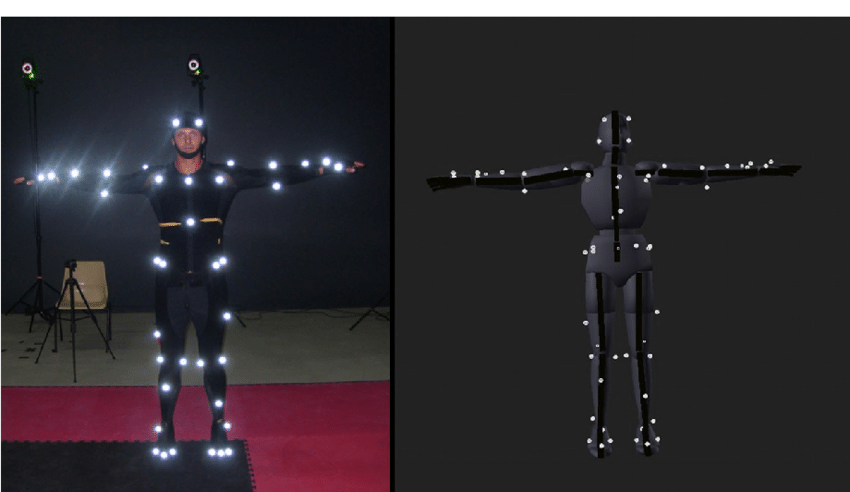
\includegraphics[width=0.6\textwidth]{figures/background/Optical.png}
	\captionsetup{labelformat=empty}
	\caption{\href{https://www.researchgate.net/profile/Jacek-Hordyj/publication/283152771/figure/fig1/AS:669997391159296@1536751234023/Actor-wearing-suit-adjusted-for-optical-motion-capture-on-the-left-Virtual-model.png}
	{Optical Motion Capture suit}}
\end{figure}

Multiple high-speed cameras   \cite{Optical Motion Capture: Theory and Implementation,MOTION CAPTURE TO BUILD A FOUNDATION FOR A COMPUTER-CONTROLLED INSTRUMENT BY STUDY OF CLASSICAL GUITAR PERFORMANCE} or video cameras are used in optical motion capture systems to triangulate the position of each marker on the actor. This method involves using a series of synchronized cameras to capture markers placed in strategic locations on the body. More specifically, a number of synchronized cameras, an image acquisition system, a capturing area, and a special suit with markers are all required for the implementation of an optical motion capture system.The positions of the markers on the suit are designed to cover the necessary body parts.\\

Passive optical marker systems employ a variety of highly reflective markers of varying sizes that reflect light back to cameras. These markers can be velcroed to a body suit or applied directly to the skin. A ring of visible red, near red, or infrared strobe light emitting diodes (LEDs) around the camera lens generates the reflected light. The cameras' light sensitivity can be adjusted to reject other sources of light. Passive markers have the advantage of not requiring a power source such as batteries, wiring, or other electronic devices. The downside is that to the cameras, all of the markings appear to be the same. This means that if many markers are occluded and subsequently reappear in camera view, the cameras are unable to distinguish between them.\\

Active optical marker systems employ powered LEDs as markers.
Unlike passive markers, which reflect light back to cameras, these markers emit their own visible red or infrared light. These markers, like passive markers, can be adhered directly to the skin or velcroed to a body suit. The advantages of active markers are that each LED modulates and emits a unique frequency, resulting in each marker being uniquely identified. The disadvantage is that each LED must be powered, which necessitates the use of wires and related devices like batteries and circuit boards.
